\subsubsection{Cơ sở hạ tầng dưới dạng mã (Infrastructure as Code - Terraform)}

Trong kỹ thuật phần mềm,
việc cấu hình
cơ sở hạ tầng theo phương pháp thủ công
thường tiềm ẩn nhiều rủi ro
gây sai sót, tốn thời gian và gặp khó khăn trong việc tái khởi tạo một cách chính xác.
Ngoài ra, việc dọn dẹp hoặc hủy bỏ tài nguyên thủ công dễ dẫn đến tình trạng sót tài nguyên, gây lãng phí và rủi ro bảo mật.
Để giải quyết triệt để vấn đề này, phương pháp Cơ sở hạ tầng dưới dạng mã (Infrastructure as Code - IaC)
đã được áp dụng để khắc phục vấn đề đó.

Trong phạm vi đồ án này,
em sử dụng Terraform
để quản lý cấu hình một số hạ tầng của các nhà cung cấp
có hỗ trợ terraform giúp định nghĩa
và quản lý hạ tầng của dự án một cách tự động thay
vì thao tác thủ công.

\begin{figure}[H]
\centering
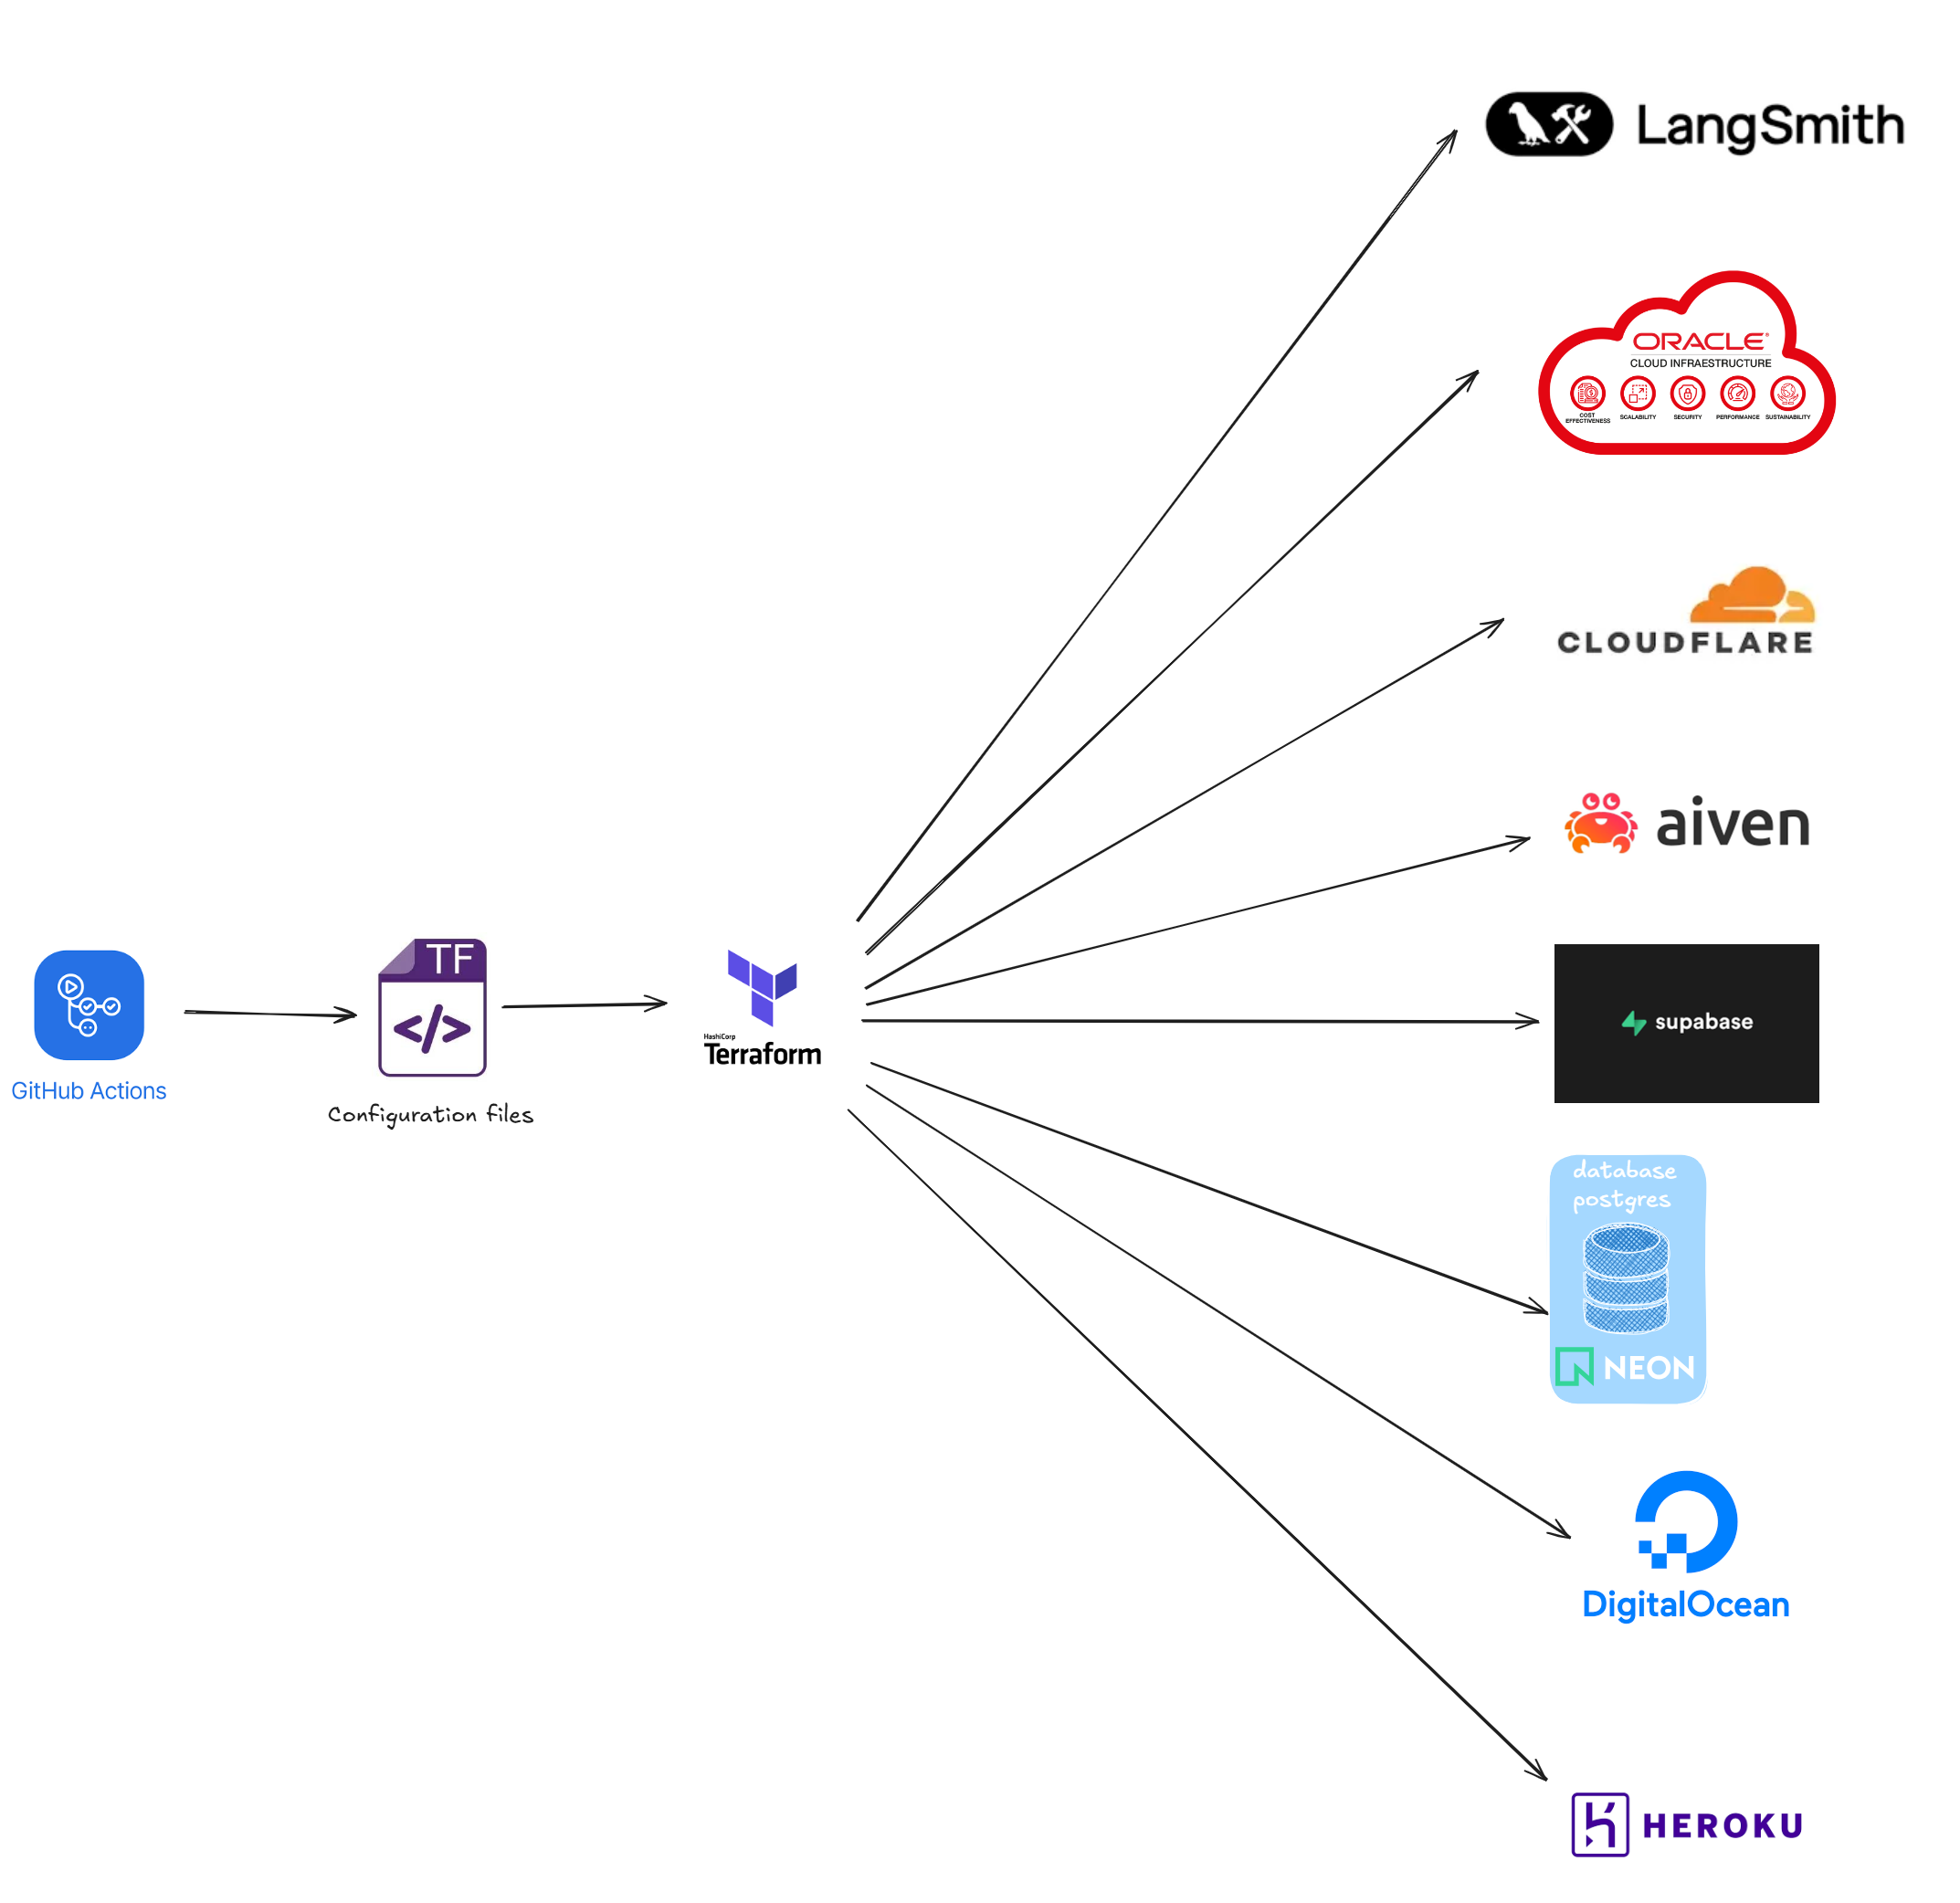
\includegraphics[scale = 0.1]{pictures/infrastructure-as-code-IaC-terraform.excalidraw.png}
\caption{Sơ đồ tổng quan quản lý hạ tầng bằng Terraform trong dự án}
\label{fig:terraform-overview}
\end{figure}

Hạ tầng của hệ thống quản lý qua các dịch vụ bao gồm:

\begin{itemize}
\item \textbf{Oracle Cloud Infrastructure (OCI):} Khởi tạo và quản lý máy chủ ảo (VPS) phục vụ triển khai ứng dụng.
\item \textbf{Aiven:} Khởi tạo cụm trung chuyển tin nhắn Kafka cho kiến trúc hướng sự kiện.
\item \textbf{Supabase:} Cấu hình hệ thống và các chính sách cho dịch vụ xác thực người dùng (Auth Service).
\item \textbf{LangSmith:} Quản lý các tài nguyên phục vụ giám sát và đánh giá chuỗi RAG (LangChain, LangGraph).
\item \textbf{Cloudflare:} Quản lý cấu hình DNS, lưu trữ đối tượng (Cloudflare R2 Bucket) và thiết lập các đường truyền an toàn (Cloudflare Tunnel).
\item \textbf{Neon:} Khởi tạo và quản lý các CSDL PostgreSQL độc lập cho từng vi dịch vụ (Microservices).
\item \textbf{DigitalOcean:} Cấu hình CSDL PostgreSQL phục vụ riêng cho luồng thu thập dữ liệu (Data Pipeline VBPL).
\item \textbf{Heroku:} Triển khai và quản lý môi trường cho dịch vụ thanh toán (Payment Service).
\end{itemize}

Ban đầu, dự án tại kho lưu trữ \url{https://github.com/20206205Tech/infra-by-terraform} sử dụng mô hình một \textit{Root Module} lớn để truyền biến vào các module con nằm trong thư mục \texttt{modules/}. Tuy nhiên, mô hình này bộc lộ một số hạn chế khi chạy CI/CD: quy trình dễ bị gián đoạn nếu một \textit{provider} gặp sự cố cục bộ, hoặc gây lãng phí thời gian khi hệ thống bắt buộc phải thực hiện lệnh \texttt{terraform init} cho toàn bộ các \textit{provider} mặc dù chỉ có một thay đổi rất nhỏ ở một dịch vụ cụ thể.

Để khắc phục nhược điểm trên, cấu trúc hạ tầng đã được tái cấu trúc lại tại kho lưu trữ \url{https://github.com/20206205Tech/infrastructure}. Tại đây, mỗi \textit{provider} được cô lập trong một thư mục riêng biệt. Đồng thời, hệ thống kết hợp với GitOps thông qua GitHub Actions, cho phép chỉ kích hoạt quy trình kiểm tra và triển khai Terraform khi và chỉ khi có sự thay đổi dữ liệu bên trong thư mục của \textit{provider} tương ứng.

\begin{figure}[H]
\centering
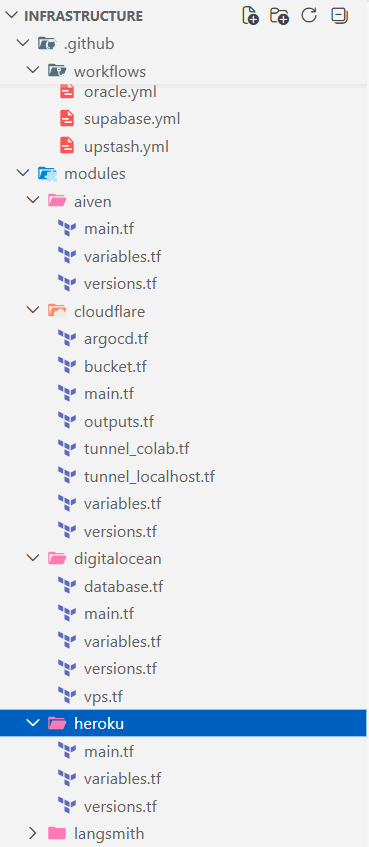
\includegraphics[scale = 0.2]{pictures/infrastructure-project-v2.png}
\caption{Cấu trúc thư mục dự án Terraform cải tiến theo từng Provider}
\label{fig:terraform-structure}
\end{figure}

Bên cạnh đó, dự án sử dụng giải pháp Terraform Cloud đóng vai trò làm \textit{Remote Backend} để lưu trữ trạng thái (\textit{State File}) tập trung và an toàn, hỗ trợ cơ chế khóa trạng thái (\textit{State Locking}) nhằm tránh xung đột khi có nhiều tiến trình cùng ghi dữ liệu.

\begin{figure}[H]
\centering
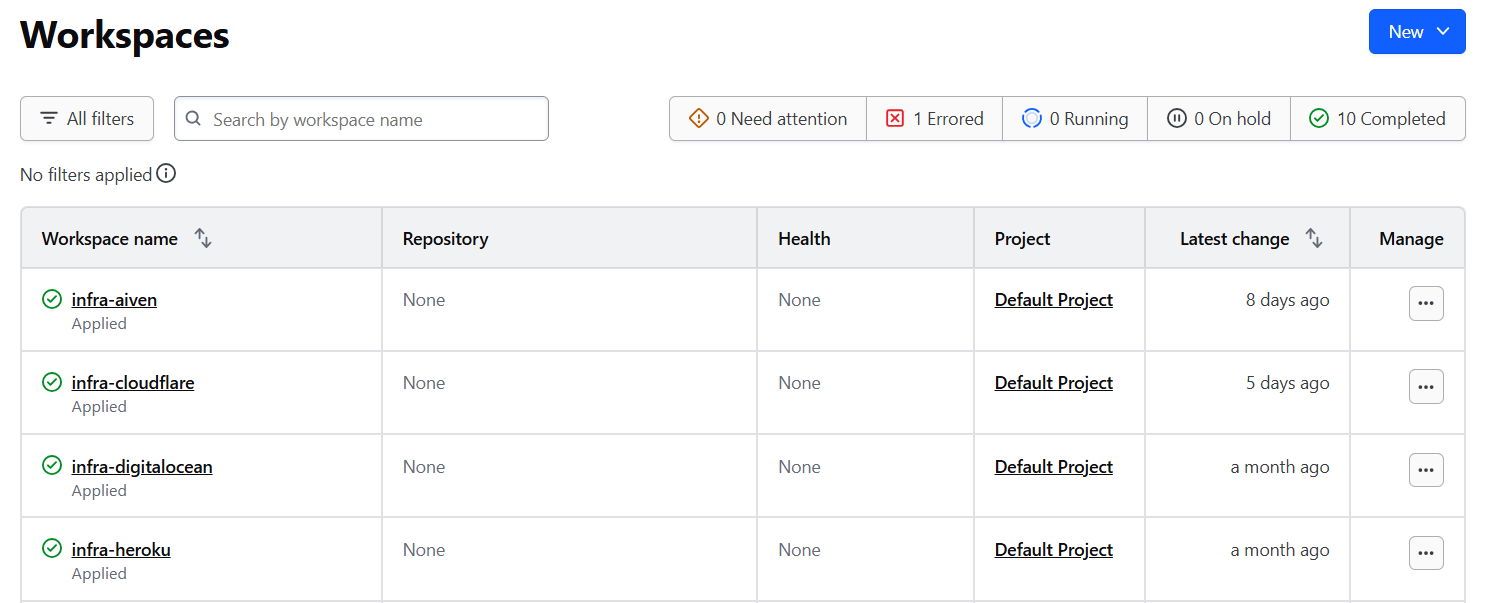
\includegraphics[scale = 0.2]{pictures/terraform-hub-web-ui.png}
\caption{Giao diện quản lý trạng thái tập trung trên Terraform Cloud}
\label{fig:terraform-cloud}
\end{figure}

Dưới đây là kết quả thực tế các tài nguyên được khởi tạo tự động thông qua mã nguồn Terraform thành công:

\begin{figure}[H]
\centering
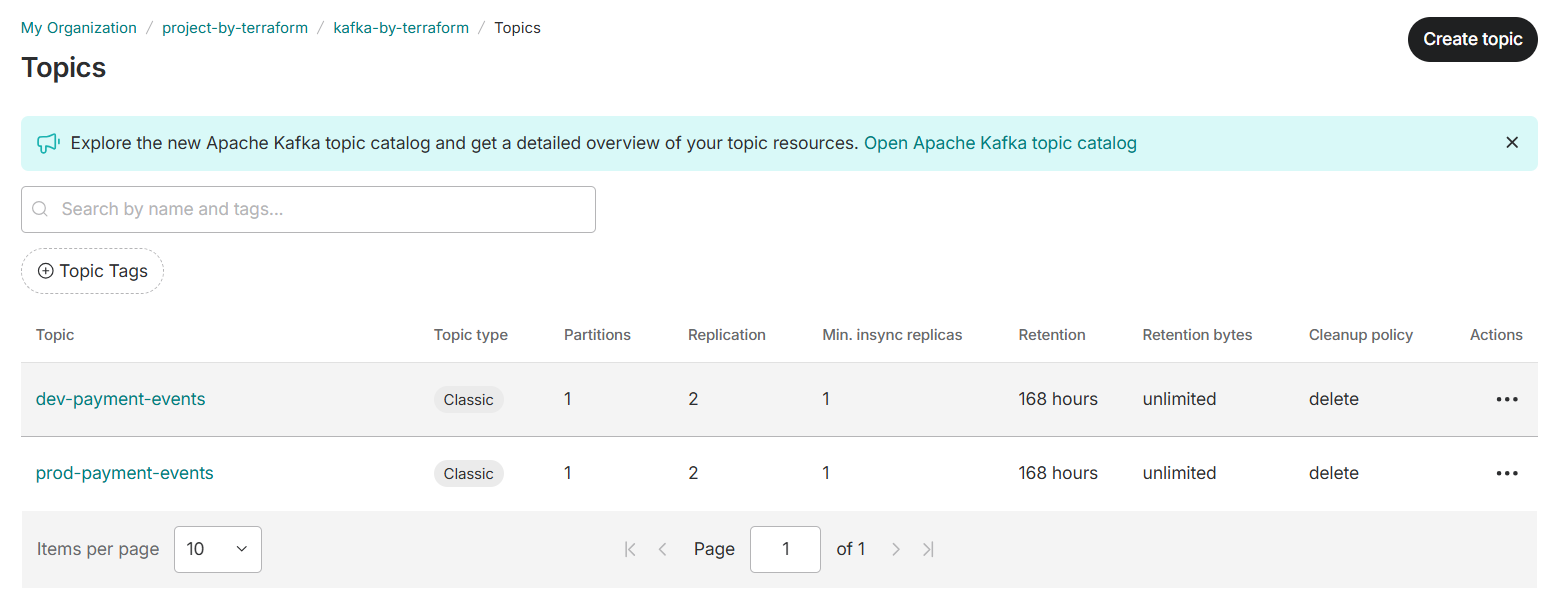
\includegraphics[scale = 0.2]{pictures/kafka-aiven-terraform.png}
\caption{Cụm dịch vụ Kafka trên nền tảng Aiven được cấu hình tự động}
\label{fig:kafka-aiven}
\end{figure}

\begin{figure}[H]
\centering
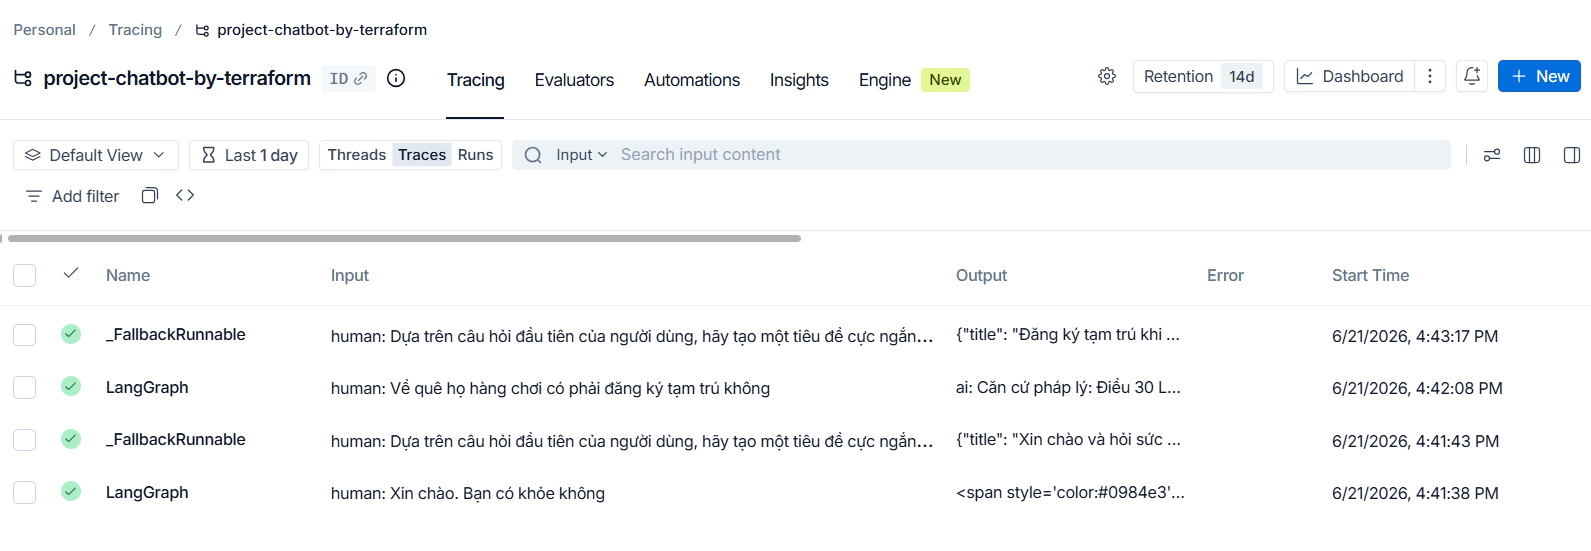
\includegraphics[scale = 0.2]{pictures/langsmith-terraform.png}
\caption{Không gian làm việc (Workspace) LangSmith được khởi tạo qua mã nguồn}
\label{fig:langsmith-tf}
\end{figure}

\begin{figure}[H]
\centering
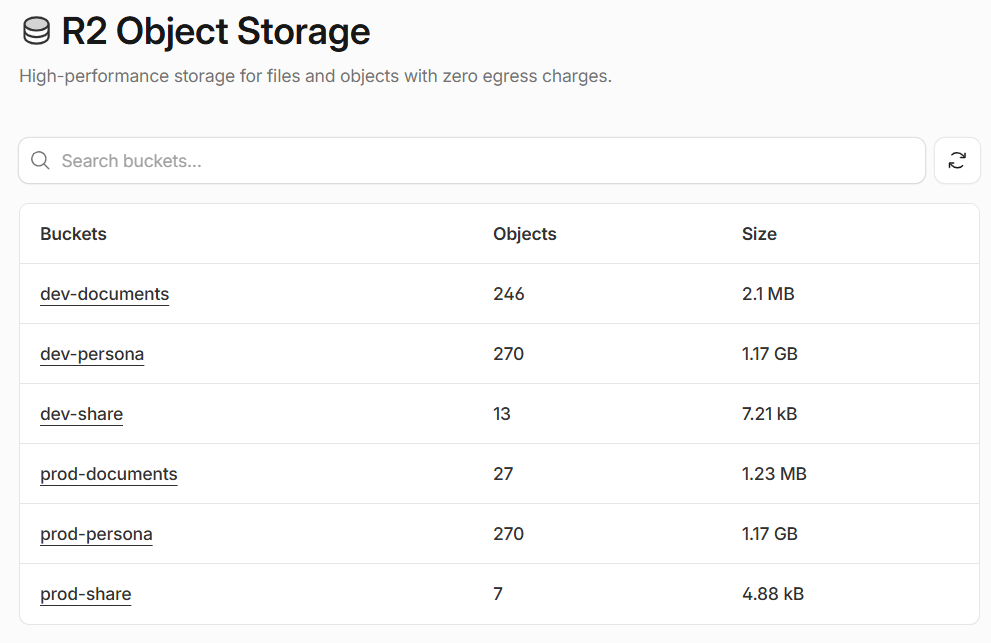
\includegraphics[scale = 0.2]{pictures/cloudflare-r2-terraform.png}
\caption{Cấu hình các R2 Bucket thành công trên Cloudflare}
\label{fig:cloudflare-r2}
\end{figure}

Do chính sách tài khoản miễn phí của Neon có nhiều giới hạn về tài nguyên (như số lượng database, compute hours), trong mã nguồn Terraform, em đã cấu hình tách biệt hoàn toàn thành các dự án (\textit{Project}) riêng lẻ trên Neon cho từng môi trường/dịch vụ nhằm tối ưu hóa hạn mức và đảm bảo tính độc lập dữ liệu.

\begin{figure}[H]
\centering
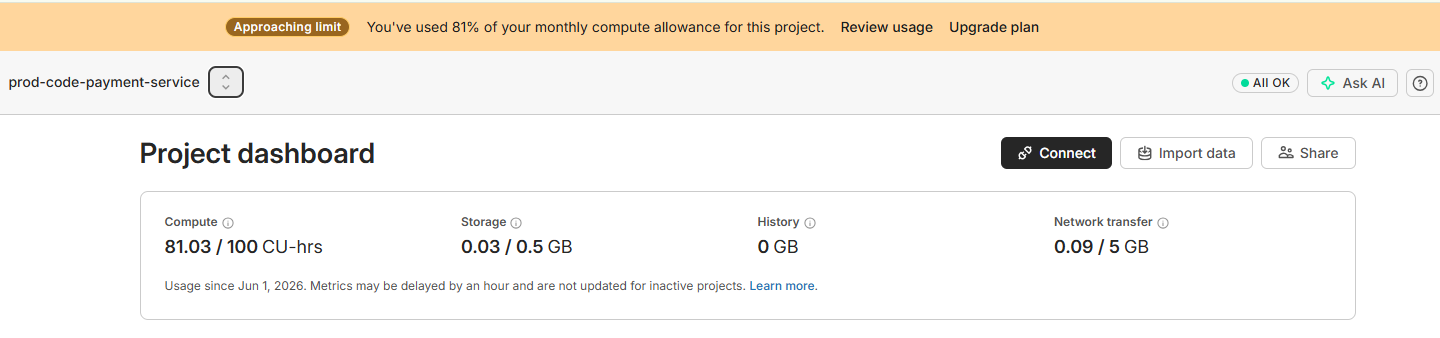
\includegraphics[scale = 0.2]{pictures/neon-limit-free.png}
\caption{Giao diện giám sát giới hạn tài nguyên của tài khoản miễn phí trên Neon}
\label{fig:neon-limit}
\end{figure}
